\section{Error analysis and shortcut re-check}

Gate G4 global heads (\texttt{indomain\_\allowbreak{}e2s}, EMA) on the validation rows; the locked test numbers are in P090. Run \texttt{20261105T135840Z\_\allowbreak{}error\_\allowbreak{}analysis\_\allowbreak{}8ac9f81ffc}.

\subsection{Genus confusions (native classes)}

\begin{figure}[h]
\centering
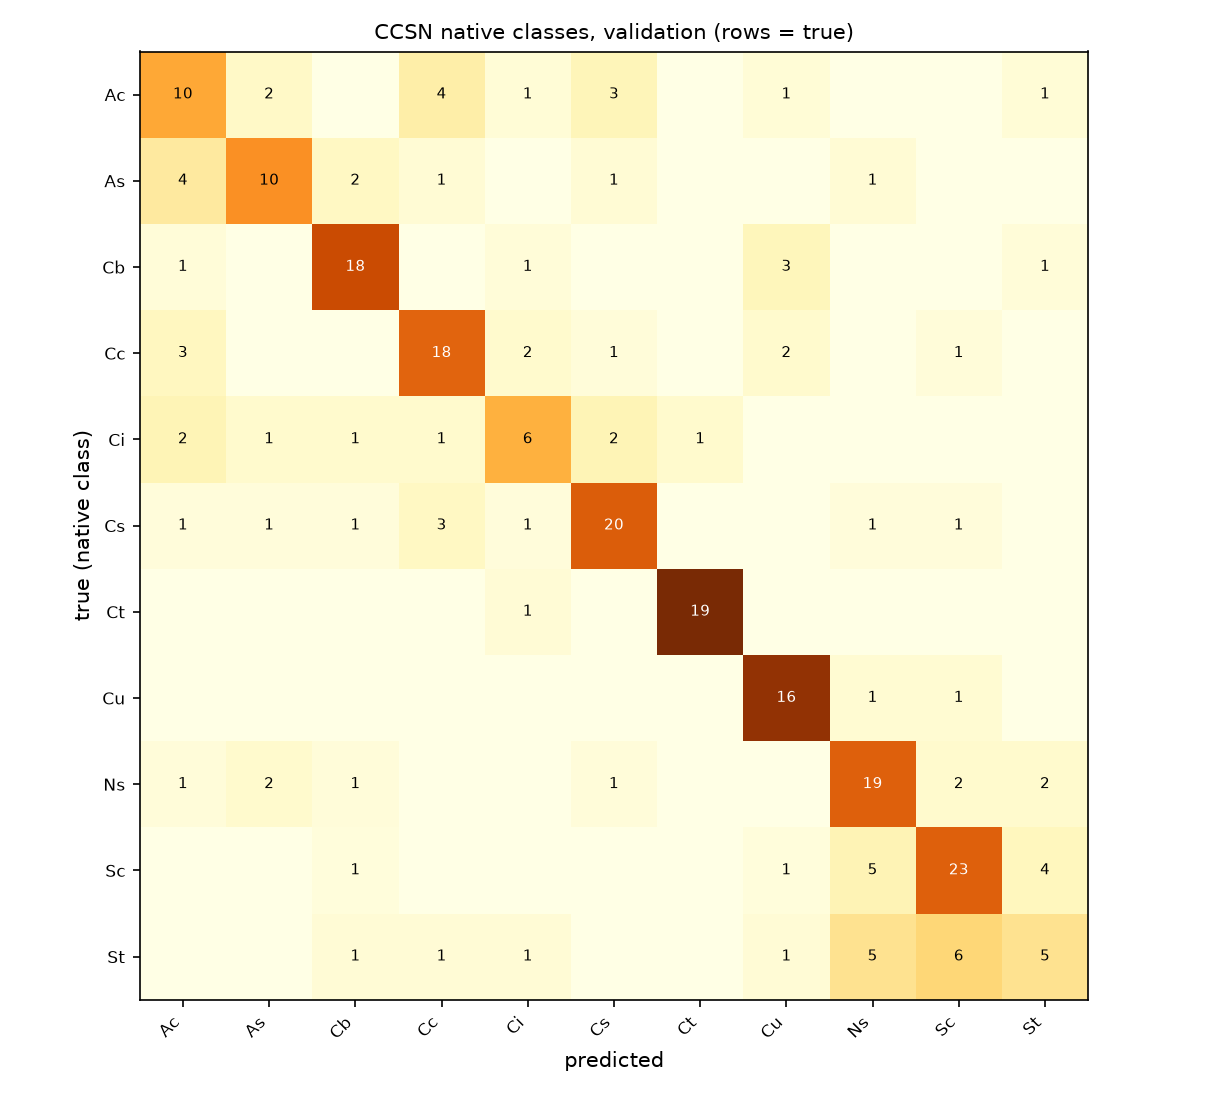
\includegraphics[width=0.9\linewidth]{supp/fig/genus_confusion_ccsn.png}
\caption{CCSN}
\end{figure}

\begin{figure}[h]
\centering
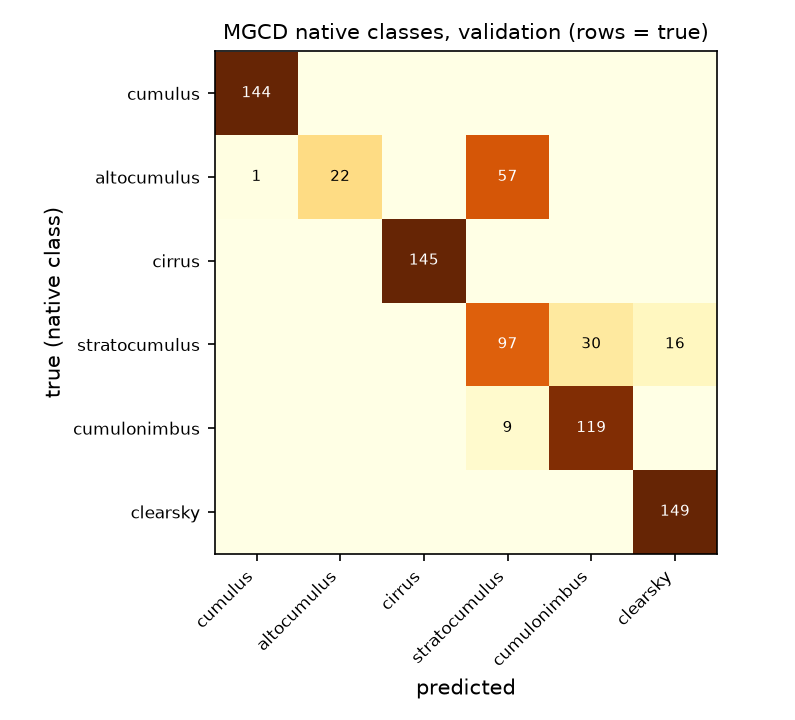
\includegraphics[width=0.9\linewidth]{supp/fig/genus_confusion_mgcd.png}
\caption{MGCD}
\end{figure}

\begin{center}{\scriptsize\setlength{\tabcolsep}{3pt}
\begin{tabular}{lllll}
\toprule
Dataset & Class & Recall & n & Most confused with (share) \\
\midrule
CCSN & all & accuracy 0.643 & 255 &  \\
CCSN & Ac & 0.455 & 22 & Cc (0.18) \\
CCSN & As & 0.526 & 19 & Ac (0.21) \\
CCSN & Cb & 0.750 & 24 & Cu (0.12) \\
CCSN & Cc & 0.667 & 27 & Ac (0.11) \\
CCSN & Ci & 0.429 & 14 & Cs (0.14) \\
CCSN & Cs & 0.690 & 29 & Cc (0.10) \\
CCSN & Ct & 0.950 & 20 & Ci (0.05) \\
CCSN & Cu & 0.889 & 18 & Ns (0.06) \\
CCSN & Ns & 0.679 & 28 & St (0.07) \\
CCSN & Sc & 0.676 & 34 & Ns (0.15) \\
CCSN & St & 0.250 & 20 & Sc (0.30) \\
MGCD & all & accuracy 0.857 & 789 &  \\
MGCD & cumulus & 1.000 & 144 &  \\
MGCD & altocumulus & 0.275 & 80 & stratocumulus (0.71) \\
MGCD & cirrus & 1.000 & 145 &  \\
MGCD & stratocumulus & 0.678 & 143 & cumulonimbus (0.21) \\
MGCD & cumulonimbus & 0.930 & 128 & stratocumulus (0.07) \\
MGCD & clearsky & 1.000 & 149 &  \\
\bottomrule
\end{tabular}}
\end{center}

\begin{center}{\scriptsize\setlength{\tabcolsep}{3pt}
\begin{tabular}{llp{12.6cm}ll}
\toprule
Dataset & Pair & Swapped share of the pair's rows & n & Counts \\
\midrule
CCSN & St/Sc & 0.185 & 54 & 6 St-$>$Sc, 4 Sc-$>$St \\
CCSN & Ci/Cs & 0.070 & 43 & 2 Ci-$>$Cs, 1 Cs-$>$Ci \\
CCSN & As/Ns & 0.064 & 47 & 1 As-$>$Ns, 2 Ns-$>$As \\
\bottomrule
\end{tabular}}
\end{center}

\subsection{Étage presence per source (exhaustive étage rows, threshold 0.5)}

\begin{center}{\scriptsize\setlength{\tabcolsep}{3pt}
\begin{tabular}{llllll}
\toprule
Source & Étage & True rate & Predicted rate & Missed & Spurious \\
\midrule
almeria & low & 0.429 & 0.583 & 0.111 & 0.354 \\
almeria & mid & 0.464 & 0.321 & 0.410 & 0.089 \\
almeria & high & 0.321 & 0.250 & 0.222 & 0.000 \\
almeria & exact set & 0.607 &  &  &  \\
ccsn & low & 0.386 & 0.407 & 0.110 & 0.103 \\
ccsn & mid & 0.263 & 0.212 & 0.355 & 0.057 \\
ccsn & high & 0.267 & 0.267 & 0.175 & 0.064 \\
ccsn & exact set & 0.771 &  &  &  \\
mgcd & low & 0.329 & 0.329 & 0.000 & 0.000 \\
mgcd & mid & 0.000 & 0.000 & 0.000 & 0.000 \\
mgcd & high & 0.331 & 0.331 & 0.000 & 0.000 \\
mgcd & exact set & 1.000 &  &  &  \\
montenegro & low & 0.609 & 0.591 & 0.051 & 0.035 \\
montenegro & mid & 0.022 & 0.020 & 0.455 & 0.008 \\
montenegro & high & 0.057 & 0.102 & 0.241 & 0.062 \\
montenegro & exact set & 0.892 &  &  &  \\
\bottomrule
\end{tabular}}
\end{center}

\subsection{Sun glare}

\begin{center}{\scriptsize\setlength{\tabcolsep}{3pt}
\begin{tabular}{lp{12.3cm}ll}
\toprule
Where & Quantity & Value & Clean \\
\midrule
val (P088 corruption) & etage\_f1: clean -$>$ sun glare & 0.760 & 0.838 \\
val (P088 corruption) & genus\_f1: clean -$>$ sun glare & 0.656 & 0.703 \\
val (P088 corruption) & sky\_miou: clean -$>$ sun glare & 0.816 & 0.901 \\
val (P088 corruption) & clear\_sky\_cloud\_fraction: clean -$>$ sun glare & 0.467 & 0.292 \\
val (P088 corruption) & cbh\_mae\_m: clean -$>$ sun glare & 745.508 & 605.748 \\
b0268 (adaptation days) & glare\_fraction\_strong\_frames & 0.000 & - \\
b0268 (adaptation days) & glare\_fraction\_other\_frames & 0.000 & - \\
\bottomrule
\end{tabular}}
\end{center}

\subsection{Failure gallery}

The validation frames with the largest étage error (exhaustive étage rows), true and predicted étages under each frame.

\begin{figure}[h]
\centering
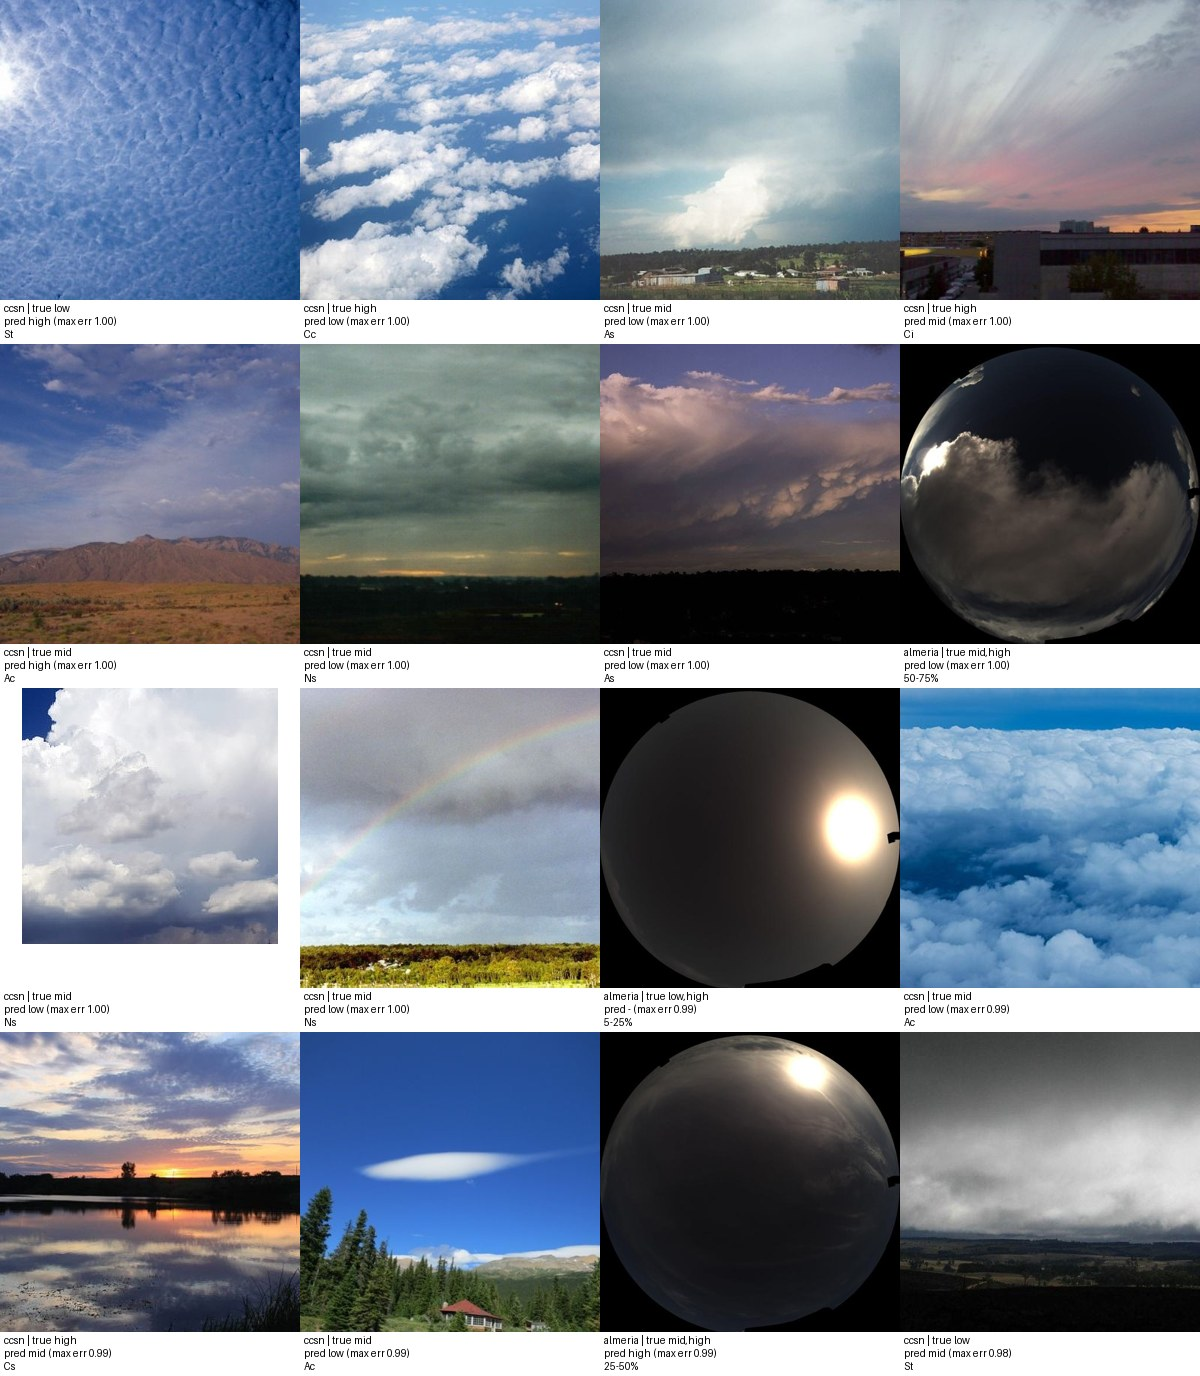
\includegraphics[width=0.9\linewidth]{supp/fig/failure_gallery.jpg}
\caption{gallery}
\end{figure}

\subsection{Dataset identity from the model's features (P029 re-check)}

\begin{center}{\scriptsize\setlength{\tabcolsep}{3pt}
\begin{tabular}{p{4.0cm}p{7.2cm}llll}
\toprule
Features & Datasets & Accuracy & Chance & n test & Note \\
\midrule
model pooled features (512-d) & eye2sky\_cbh, mgcd, montenegro, ccsn, almeria, swimcat & 1.000 & 0.167 & 131 & balanced accuracy 1.000 \\
backbone CLS features (384-d) & eye2sky\_cbh, mgcd, montenegro, ccsn, almeria, swimcat & 1.000 & 0.167 & 131 & balanced accuracy 1.000 \\
\bottomrule
\end{tabular}}
\end{center}

Attention maps were not produced: the heads pool an 8 $\times$ 8 token grid through a learned attention pool whose weights are not stored at inference; the sky-parse mask is the per-pixel view the paper shows instead.

